\chapter{Domain}
\label{chap:domain}

This chapter begins with an high level description of the domain. This is followed by a description of the schema in the relational database of CIMS and its use cases.
\begin{figure}[h!]
\centering
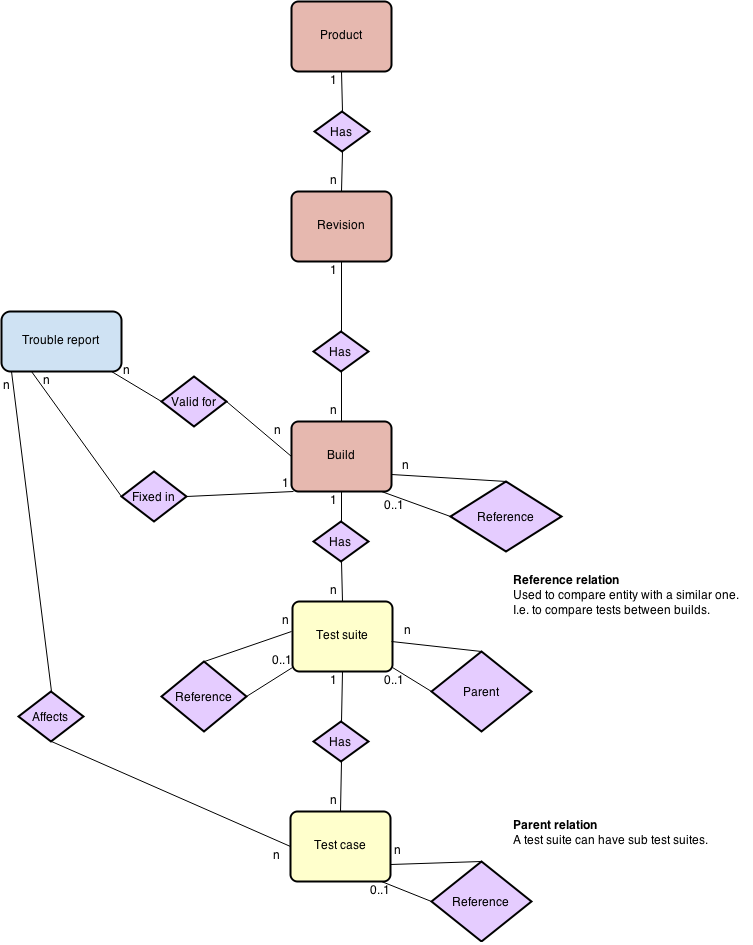
\includegraphics[scale=0.5]{figure/er_diagram.png}
\caption{High level diagram of the domain.}
\label{fig:er}
\end{figure}

\section{High level schema}
The domain in which CIMS operates has the following high level entities; products, revisions, builds, test suites, test cases and trouble reports. Excluding trouble reports, these entities form a hierarchical structure as seen in figure~\ref{fig:er}. Products are at the top of this hierarchy. They represent the different software systems that are being developed at Ericsson. Products are developed iteratively, where each released iteration is called a revision. At the revision level, developers makes changes to source code, configuration, tests etc.\ which are then checked into a revision control system and subsequently built and tested. This is referred to in domain terms as a build. Each build runs a number of test suites, which in turn consist of a number test cases.

As has been noted, a trouble report sits outside of the hierarchy. This entity represents a bug or defect which arrives from external (i.e.\ a customer) or internal sources. It can be mapped to different entities from products down to specific test cases. Trouble reports are handled by implementing a fix in a specific build.

\section{Existing relational implementation}
The relational database schema in use by CIMS represents the above mentioned entities in a different abstraction. Representation of these entities are described in depth in the sections below. 
The schema of the relational database in CIMS is presented in figure~\ref{fig:sql}.
\hiddensubsection{Test suite}
\begin{figure}[h!]
\centering
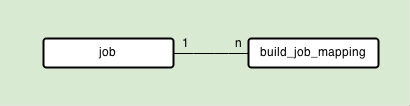
\includegraphics[scale=0.5]{figure/job.jpg}
\caption{Diagram of tables related to test suites.}
\label{fig:job}
\end{figure}
The top level entity of a test suite is represented by the job table. A job is used to group related job events and thereby form a test suite. A test suite is run within a build, as seen in figure~\ref{fig:job}, a job belongs to a build via the 'build job mapping' table. 
\hiddensubsection{Build}
\begin{figure}[h!]
\centering
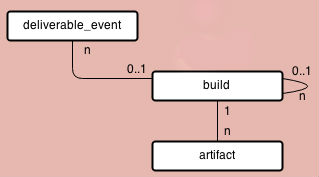
\includegraphics[scale=0.5]{figure/build.jpg}
\caption{Diagram of tables related to builds.}
\label{fig:build}
\end{figure}
In the relational database, a build is represented by the build table. Each build can posses a number of artifacts and deliverable\_events, as seen in figure~\ref{fig:build}. An artifact can be whatever we want...
\hiddensubsection{Test case}
\begin{figure}[h!]
\centering
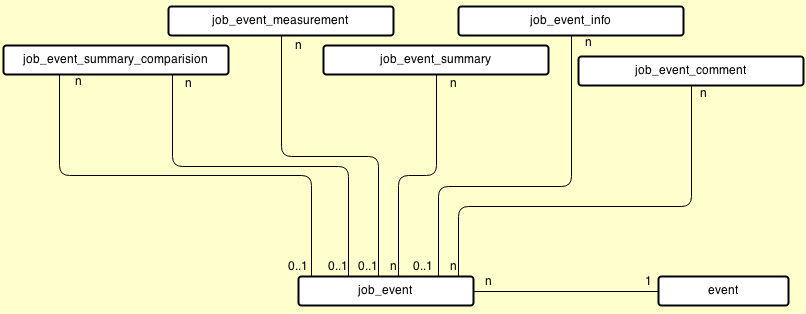
\includegraphics[scale=0.5]{figure/job_event.jpg}
\caption{Diagram of tables related to test cases.}
\label{fig:job_event}
\end{figure}

\hiddensubsection{Deliverable}
\begin{figure}[h!]
\centering
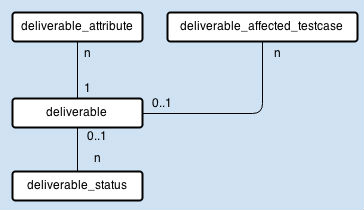
\includegraphics[scale=0.5]{figure/deliverable.jpg}
\caption{Diagram of tables related to trouble reports.}
\label{fig:deliverable}
\end{figure}


\section{Use cases}
\label{sec:usecases}
The set of queries that the archive should support is presented in the following sections. They are described in domain terms and in terms of the relational implementation of CIMS.

%table~\ref{tab:queries}.

\begin{figure}[h!]
\centering
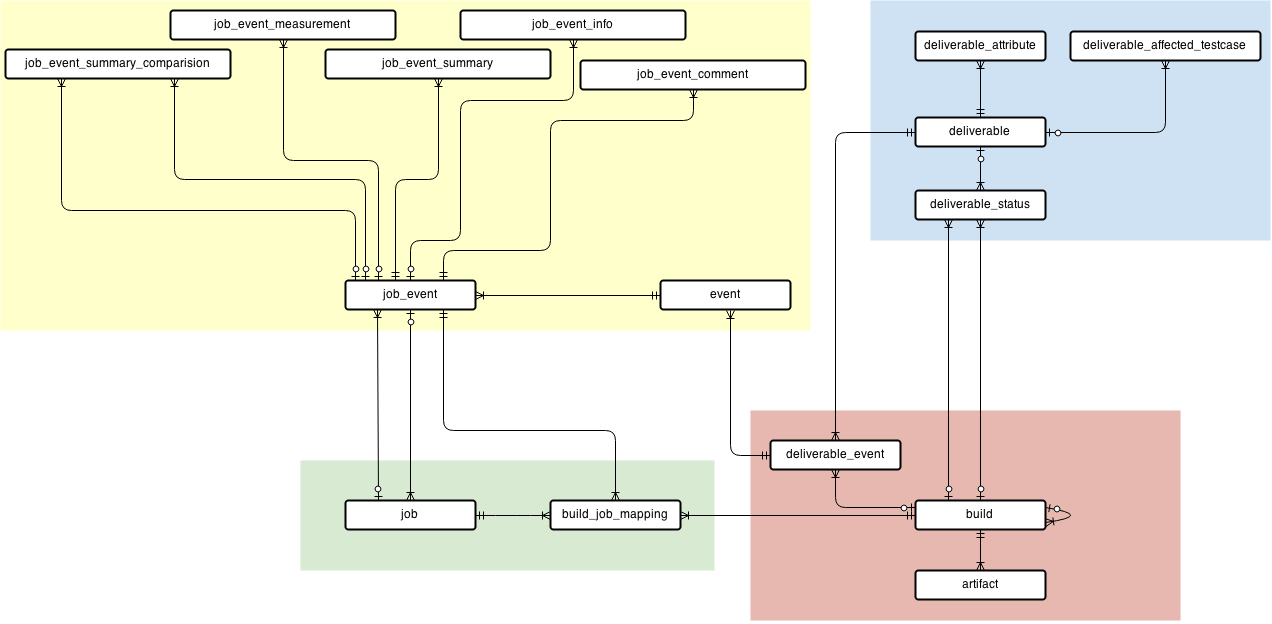
\includegraphics[scale=0.5, angle=90]{figure/sql.png}
\caption{Diagram of the relational database in CIMS.}
\label{fig:sql}
\end{figure}

%\begin{table}[h]
%\begin{tabular}{|l|l|}
%\hline
%\textbf{High level query}                & \textbf{Query in CIMS}                    \\ \hline
%Get build                                    & Get build by id                           \\ \hline
%Get build information                        & Get build information by id               \\ \hline
%Get build for root test suite                & Get build by simple id                    \\ \hline
%Get trouble reports for build                & Get deliverables for build                \\ \hline
%Get trouble report fixes for build           & Get deliverables for build                \\ \hline
%Get trouble reports for product and revision & Get deliverables for product and revision \\ \hline
%Get test suite children                      & Get job event children                    \\ \hline
%Get test case in build                       & Get job event by id                       \\ \hline
%Get test suite in build                      & Get job event by id                       \\ \hline
%Get root test suite for test case/test suite & Get root job event                        \\ \hline
%Get test case by name                        & Get job event by name                     \\ \hline
%Get test suite for test case                 & Get parent job event                      \\ \hline
%Get test case history                        & Get event history                         \\ \hline
%Get test tree                                & Get job tree by id                        \\ \hline
%\end{tabular}
%\caption{Set of important queries on the relational database of CIMS}
%\label{tab:queries}
%\end{table}

\hiddensubsection{Get build}
\label{q:getbuild}
Query in CIMS: Get build by id \\
SQL: {\tt SELECT * FROM cims\_build WHERE id = 'some\_id'} \\
Example input: {\tt CXS101289\_LLVDRAGON\_MKX\_SPRINT3\_R1A03\_140605084139 } \\
Example output: \\
This query is simply used to uniquely identify a build.

\hiddensubsection{Get build information}
\label{q:getbuildinfo}
Query in CIMS: Get build information by id \\
SQL: {\tt SELECT product\_name, product\_revision, verdict, start, end FROM cims\_build WHERE id = 'some\_id'} \\
Example input: {\tt CXS101289\_LLVDRAGON\_MKX\_SPRINT3\_R1A03\_140605084139 }  \\
Example output: \\
Given a unique build id, return the basic information for that build, i.e. product, revision, verdict, start/stop times.

\hiddensubsection{Get build for root test suite}
\label{q:getbuildforroot}
Query in CIMS: Get build by job event simple id \\
SQL: 
\begin{verbatim}
SELECT cims_build.* FROM cims_build
INNER JOIN cims_build_job_mapping
ON cims_build_job_mapping.build_id = cims_build.id   
WHERE cims_build_job_mapping.job_id = 'some_simple_id'
\end{verbatim} 
Example input: {\tt 1234567 }  \\
Example output: \\
This query should retrieve the build that a root test suite belongs to.

%\hiddensubsection{Get trouble reports for build}
%\label{q:getrforbuild}
%Query in CIMS: Get deliverables for build \\
%Example input: {\tt CXS101289\_LLVDRAGON\_MKX\_SPRINT3\_R1A03\_140605084139 }  \\
%Example output: \\
%Given a unique build id, return a list of deliverables valid for that build. In domain terms this means %retrieving all trouble reports that affect the build.

%\hiddensubsection{Get trouble report fixes for build}
%\label{q:getrfixforbuild}
%Query in CIMS: Get deliverables for build \\
%Example input: {\tt CXS101289\_LLVDRAGON\_MKX\_SPRINT3\_R1A03\_140605084139 }  \\
%Example output: \\
%Given a unique build id, retrieve all trouble report fixes that the build delivered.

%\hiddensubsection{Get trouble reports for product and revision}
%\label{q:gettrforprod}
%Query in CIMS: Get deliverables for product and revision \\%%Example input: {\tt (Product=ndpgsn\_5\_0\_llvdragon\_mkx\_sprint3,\ Revision=R1A03) }  \\
%Example output: \\
%Given a combination of a product name and a revision name, return a list of deliverables that affect that combination. In domain terms this means returning trouble reports that affect the combination.

%\hiddensubsection{Get test suite children}
%\label{q:gettestsuitechildren}
%Query in CIMS: Get job event children \\
%SQL: {\tt SELECT * FROM cims\_job\_event WHERE parent\_jobevent\_id = 'some\_id' }
%Example input: {\tt fff70f3a-c69e-44c1-b9f5-7e5ae5a59610 } \\
%Example output: \\
%For implementational reasons, both test cases and test suites are represented as job events in the relational data model of CIMS. As such, a job event id uniquely identifies a specific test case or test suite in a specific build. This query should, given a job event id, return its children. In domain terms this means that for a specific build, return the child nodes of a test suite. These child nodes can be test cases (leaf nodes) or test suites (tree nodes).

%\hiddensubsection{Get test case in build}
%\label{q:gettcinbuild}
%Query in CIMS: Get job event by id \\
%SQL: {\tt SELECT * FROM cims\_job\_event WHERE id = 'some\_id' } \\
%Example input: {\tt fff70f3a-c69e-44c1-b9f5-7e5ae5a59610 } \\%%Example output: \\
%This query should retrieve information about a test case in a specific build. In the relational data model of CIMS this can be translated to retrieving a job event by its unique id.

%\hiddensubsection{Get test suite in build}
%\label{q:gettcinbuild}
%Query in CIMS: Get job event by id \\
%SQL: {\tt SELECT * FROM cims\_job\_event WHERE id = 'some\_id' } \\
%Example input: {\tt fff70f3a-c69e-44c1-b9f5-7e5ae5a59610 } \\
%Example output: \\
%This query should retrieve information about a test suite in a specific build. In CIMS, test suites and test cases are both represented by the job event entity and as such the query in CIMS is the same as the previous query.

\hiddensubsection{Get root test suite for test case/test suite}
\label{q:getrootts}
Query in CIMS: Get root job event \\
SQL:
\begin{verbatim}
SELECT cims_job_event.* FROM cims_job
INNER JOIN cims_job_event ON cims_job_event.id = cims_job.root_jobevent_id
WHERE cims_job.job_name =
(SELECT job_name FROM cims_job_event WHERE id = 'some_id')

\end{verbatim}
Example input: {\tt fff70f3a-c69e-44c1-b9f5-7e5ae5a59610 } \\
Example output: \\
Given the unique id of a test case or test suite, this query should retrieve the related root test suite.

\hiddensubsection{Get test case by name}
\label{q:gettcbyname}
Query in CIMS: Get job event by name \\
SQL: {\tt SELECT * FROM cims\_job\_event WHERE name = 'some\_name' } \\
Example input: {\tt tc\_48\_027\_handover\_roaming\_restricted } \\
Example output: \\
Every test case has a descriptive name. This query should retrieve all test cases with a given name. This means retrieving test cases from different builds, since builds often share the same test suites and test cases.

%\hiddensubsection{Get test suite for test case}
%\label{q:gettsfortc}
%Query in CIMS: Get parent job event \\
%SQL:
%\begin{verbatim}
%SELECT * FROM cims_job_event
%WHERE cims_job_event.id =
%(SELECT parent_jobevent_id FROM cims_job_event WHERE id = 'some_id')
%\end{verbatim}
%Example input: {\tt fff70f3a-c69e-44c1-b9f5-7e5ae5a59610 } \\
%Example output: \\
%For a test case in a specific build, retrieve the test suite it belongs to in that build.

\hiddensubsection{Get test case history}
\label{q:tchistory}
Query in CIMS: Get event history \\
SQL: This query cannot be expressed as a single SQL statement and is implemented on the application level in CIMS by performing several SQL queries and building a dictionary with the results. Psuedo code for query:
\begin{verbatim}
job_events = SELECT * FROM cims_job_event WHERE name = 'some_name'
job_names = job_event.job_name FOR job_event IN job_events // List comprehension

jobs = SELECT * FROM cims_job WHERE job_name IN job_names
root_job_event_ids = job.root_jobevent_id FOR job IN jobs // List comprehension
root_job_events = SELECT * FROM job_event WHERE id IN root_job_event_ids

builds = 
    SELECT cims_build.* FROM cims_build
    INNER JOIN cims_build_job_mapping
    ON cims_build_job_mapping.build_id = cims_build.id
    WHERE cims_build_job_mapping.job_name IN job_names

(Use list of job_events, jobs, root job events and builds to create result dictionary)

\end{verbatim}
Example input: {\tt tc\_48\_027\_handover\_roaming\_restricted } \\
Example output: \\
This query should return the history of a test case, identified by its name, filtered optionally by extra parameters. It should group the results by product and for each of these show the builds containing the specific test case and the verdict of the test case in that build.

%\hiddensubsection{Get test tree}
%\label{q:gettesttree}
%Query in CIMS: Get job tree by id or job name \\
%SQL: This query cannot be performed with a single SQL statement. The tree structure is built on the application level. Pseudo code:
%\begin{verbatim}
%job_events = SELECT * FROM cims_job_event WHERE job_name = 'some_name'
%create_tree_structure(job_events) // Recursive function
%\end{verbatim}
%Example input: $1234567$\\
%Example output: \\
%In the relational data model of CIMS, a job represents a root test suite for a specific build. I.e a test suite with no parent. This query should, given a unique id of such a job, return the hierarchical representation of that job.


\hiddensubsection{Get all build data}
\label{q:getallbuilddata}
Query in CIMS: na \\
SQL: This specific query is not expressed as a single SQL statement. Pseudo code:
\begin{verbatim}
build = SELECT * FROM cims_build WHERE id = 'some_id'

jobs = 
    SELECT cims_job.* FROM cims_job
    INNER JOIN cims_build_job_mapping
    ON cims_build_job_mapping = cims_build_job_mapping.job_name = job.job_name
    WHERE cims_build_job_mapping.build_id = build.id // same id as previous query
job_names = job.name FOR job IN jobs // list comprehension

job_events = SELECT * FROM cims_job_event WHERE job_name IN job_names
\end{verbatim}
Example input: {\tt CXS101289\_LLVDRAGON\_MKX\_SPRINT3\_R1A03\_140605084139 } \\
Example output: \\
This query should retrieve the complete view of a uniquely identified build. This means all the build information plus all related test suites and test cases.

%\section{Architecture of CIMS}

%CIMS has a multitier architecture as seen in figure X. Whenever a build is started, data from multiple sources is collected and sent to the system. This data is transformed to fit into the relational data model of CIMS.
%
%Presentation of data is done in real time via a web application. In order to support this, CIMS employs a number technologies in support of the main relational database, effectively forming a polyglot persistence solution. This includes a search engine (Sphinx) for aggregation of test cases, and a key value store (Redis) for caching.
%
%An external REST API is exposed to gather data for other purposes than real time visualization.